 \documentclass[a4paper]{article}

\author{Olivier Berghmans, Nick De Frangh, Dirk Delahaye,\\Kristof Overdulve, Pieter-Jan Pintens, Tobias Van Bladel}
\title{Architectuur en Algoritmen van Computer Games\\\textbf{Hovercraft Universe}\\\small{\url{http://uhasseltaacgua.googlecode.com/}}}
\pagestyle{plain}
\usepackage[dutch]{babel}
\usepackage{amsfonts}
\usepackage{graphicx}
\usepackage{url}
\usepackage{todonotes}
\usepackage{hyperref}
\hypersetup{
    bookmarks=true,         % show bookmarks bar?
    unicode=false,          % non-Latin characters in Acrobat�s bookmarks
    pdftoolbar=true,        % show Acrobat�s toolbar?
    pdfmenubar=true,        % show Acrobat�s menu?
    pdffitwindow=false,     % window fit to page when opened
    pdfstartview={FitH},    % fits the width of the page to the window
    pdftitle={Architectuur en Algoritmen van Computer Games},    % title
    pdfauthor={Olivier Berghmans, Nick De Frangh, Dirk Delahaye, Kristof Overdulve, Pieter-Jan Pintens, Tobias Van Bladel},     % author
    pdfsubject={Hovercraft Universe},   % subject of the document
    %pdfcreator={Creator},   % creator of the document
    %pdfproducer={Producer}, % producer of the document
    %pdfkeywords={keywords}, % list of keywords
    pdfnewwindow=true,      % links in new window
    colorlinks=true,       % false: boxed links; true: colored links
    linkcolor=black,          % color of internal links
    citecolor=green,        % color of links to bibliography
    filecolor=magenta,      % color of file links
    urlcolor=cyan           % color of external links
}

\begin{document}

\maketitle

\tableofcontents
\newpage

\section{Introductie}

\section{Gebruikte libraries}
\begin{itemize}
\item[\textbf{Rendering}] Ogre\footnote{\url{http://www.ogre3d.org/}}
\item[\textbf{Physics}] Havok-Physics\footnote{\url{http://www.havok.com/index.php?page=havok-physics}}
\item[\textbf{Netwerk}] ZoidCom\footnote{\url{http://www.zoidcom.com/}}
\item[\textbf{Input}] Object Oriented Input System (OIS)\footnote{\url{http://sourceforge.net/projects/wgois/}}
\item[\textbf{Geluid}] FMOD Interactive Audio Middelware\footnote{\url{http://www.fmod.org/}}
\item[\textbf{Scripting}] Lua\footnote{\url{http://www.lua.org/}} en LuaBind\footnote{\url{http://www.rasterbar.com/products/luabind.html}}
\item[\textbf{GUI}] Adobe Flash\footnote{\url{http://www.adobe.com/products/flash/}} en Hikari\footnote{\url{http://code.google.com/p/hikari-library/}}.
\end{itemize}

\section{Programmastructuur en -organisatie}
\subsection{Algemeen}
\todo{Over entiteiten, controllers, gameview, etc... Structuur uitleggen op ruwe basis van SSN'67.}
\begin{figure}
	\centering
		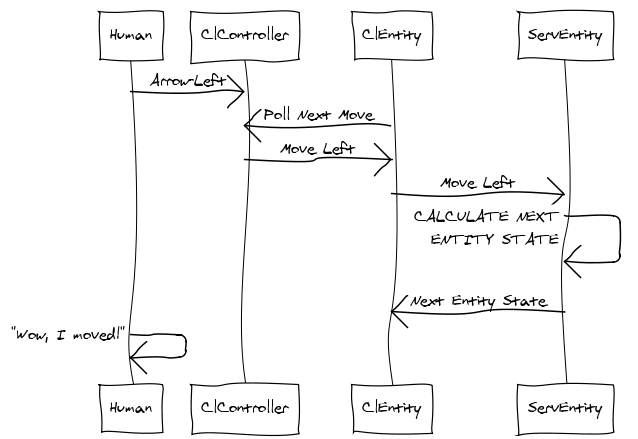
\includegraphics[width=0.50\textwidth]{images/netwerkfreq.png}
	\caption{The client entity polls its next move from the controller}
	\label{fig:netwerkfreq}
\end{figure}


\subsection{Netwerkstructuur}
\begin{figure}
	\centering
		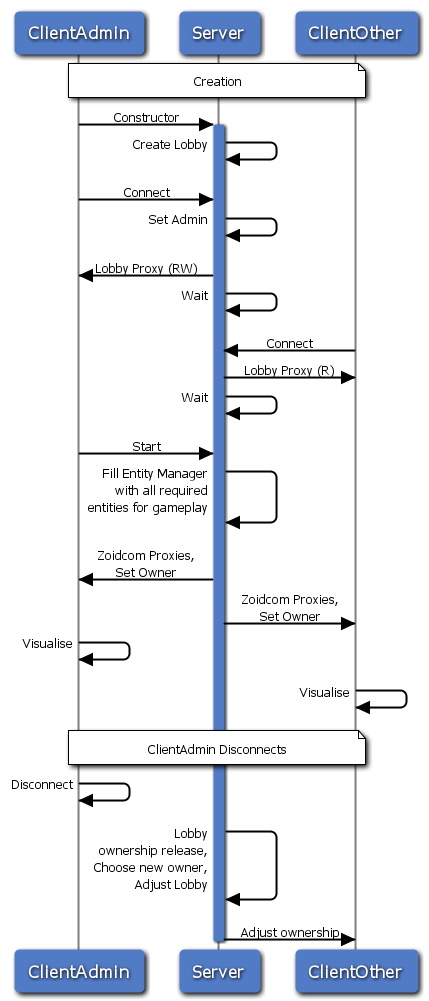
\includegraphics[width=0.50\textwidth]{images/zoidcom.png}
	\caption{ZoidCom werking}
	\label{fig:zoidcom}
\end{figure}
\todo{Over ZoidCom en het repliceren van data over het netwerk.}

\subsection{Rolverdeling en verantwoordelijkheden}
\todo{Of niet? :D}

\end{document}
